%%%%%%%%%%%%%%%%%%%%%%%%%%%%%%%%%%%%%%%%%
% Beamer Presentation
% LaTeX Template
% Version 1.0 (10/11/12)
%
% This template has been downloaded from:
% http://www.LaTeXTemplates.com
%
% License:
% CC BY-NC-SA 3.0 (http://creativecommons.org/licenses/by-nc-sa/3.0/)
%
%%%%%%%%%%%%%%%%%%%%%%%%%%%%%%%%%%%%%%%%%

%----------------------------------------------------------------------------------------
%	PACKAGES AND THEMES
%----------------------------------------------------------------------------------------

\documentclass{beamer}

\mode<presentation> {

% The Beamer class comes with a number of default slide themes
% which change the colors and layouts of slides. Below this is a list
% of all the themes, uncomment each in turn to see what they look like.

%\usetheme{default}
%\usetheme{AnnArbor}
%\usetheme{Antibes}
%\usetheme{Bergen}
%\usetheme{Berkeley}
%\usetheme{Berlin}
%\usetheme{Boadilla}
%\usetheme{CambridgeUS}
%\usetheme{Copenhagen}
%\usetheme{Darmstadt}
\usetheme{Dresden}
%\usetheme{Frankfurt}
%\usetheme{Goettingen}
%\usetheme{Hannover}
%\usetheme{Ilmenau}
%\usetheme{JuanLesPins}
%\usetheme{Luebeck}
%\usetheme{Madrid}
%\usetheme{Malmoe}
%\usetheme{Marburg}
%\usetheme{Montpellier}
%\usetheme{PaloAlto}
%\usetheme{Pittsburgh}
%\usetheme{Rochester}
%\usetheme{Singapore}
%\usetheme{Szeged}
%\usetheme{Warsaw}

% As well as themes, the Beamer class has a number of color themes
% for any slide theme. Uncomment each of these in turn to see how it
% changes the colors of your current slide theme.

%\usecolortheme{albatross}
%\usecolortheme{beaver}
%\usecolortheme{beetle}
%\usecolortheme{crane}
%\usecolortheme{dolphin}
%\usecolortheme{dove}
%\usecolortheme{fly}
%\usecolortheme{lily}
%\usecolortheme{orchid}
%\usecolortheme{rose}
%\usecolortheme{seagull}
%\usecolortheme{seahorse}
%\usecolortheme{whale}
%\usecolortheme{wolverine}

%\setbeamertemplate{footline} % To remove the footer line in all slides uncomment this line
%\setbeamertemplate{footline}[page number] % To replace the footer line in all slides with a simple slide count uncomment this line

%\setbeamertemplate{navigation symbols}{} % To remove the navigation symbols from the bottom of all slides uncomment this line
}

\usepackage{graphicx} % Allows including images
\usepackage{booktabs} % Allows the use of \toprule, \midrule and \bottomrule in tables

%----------------------------------------------------------------------------------------
%	TITLE PAGE
%----------------------------------------------------------------------------------------

\title[Design Phase]{Obstacle Avoidance and Goal Detection Robot using RPi and LRF.} % The short title appears at the bottom of every slide, the full title is only on the title page

\author{Atabak Hafeez \and
Maria Ficiu \and
Rubin Deliallisi \and
Siddharth Shukla} % Your name
\institute[Jacobs University Bremen] % Your institution as it will appear on the bottom of every slide, may be shorthand to save space
{
Jacobs University Bremen \\ % Your institution for the title page
\medskip
%\textit{john@smith.com} % Your email address
}
\date{\today} % Date, can be changed to a custom date

\begin{document}

\begin{frame}
\titlepage % Print the title page as the first slide
\end{frame}

\begin{frame}
\frametitle{Overview} % Table of contents slide, comment this block out to remove it
\tableofcontents % Throughout your presentation, if you choose to use \section{} and \subsection{} commands, these will automatically be printed on this slide as an overview of your presentation
\end{frame}


%----------------------------------------------------------------------------------------
%	PRESENTATION SLIDES
%----------------------------------------------------------------------------------------

%------------------------------------------------
\section{Introduction}
%------------------------------------------------

\subsection{Goal}
\begin{frame}
\frametitle{Goal (Basic)}
Given a goal and a robot:
\begin{itemize}
\item Turn the robot around
\item Identify the goal object from LRF input
\item Move towards the goal
\end{itemize}

\end{frame}
\begin{frame}
\frametitle{Goal (Advanced)}
Given a goal, a robot, and a maze:
\begin{itemize}
\item Turn the robot around
\item Follow the walls and avoid obstacles
\item Identify the goal from LRF input
\item Move towards the goal if nothing blocks
\end{itemize}
\end{frame}

\begin{frame}
\frametitle{Goal (Advanced)}
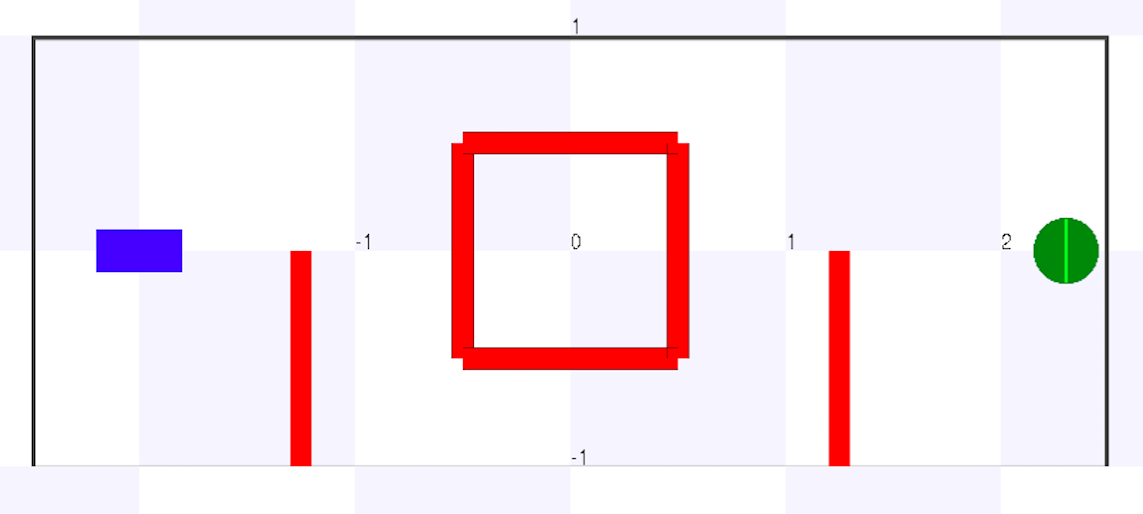
\includegraphics[scale=0.28]{assets/images/Visualization.png}
\end{frame}

\subsection{Architecture}
\begin{frame}
\frametitle{Sequence Diagram}
\begin{figure}[H]
\centering
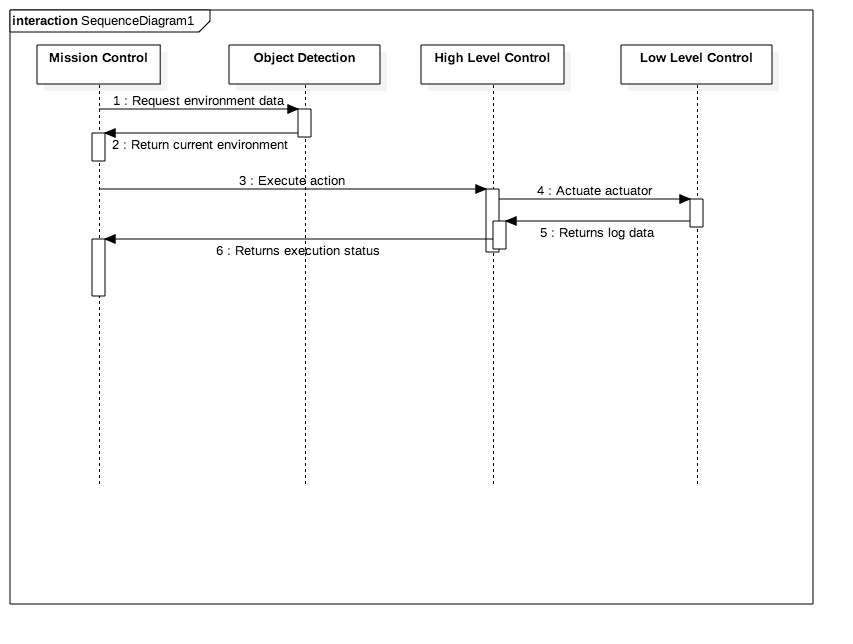
\includegraphics[scale=0.4]{assets/diagrams/SequenceDiagram.png}
%\caption{Displayes object interactions arranged in a time sequence.}
\end{figure}
\end{frame}

\begin{frame}
\frametitle{Component Diagram}
\begin{figure}[H]
\centering
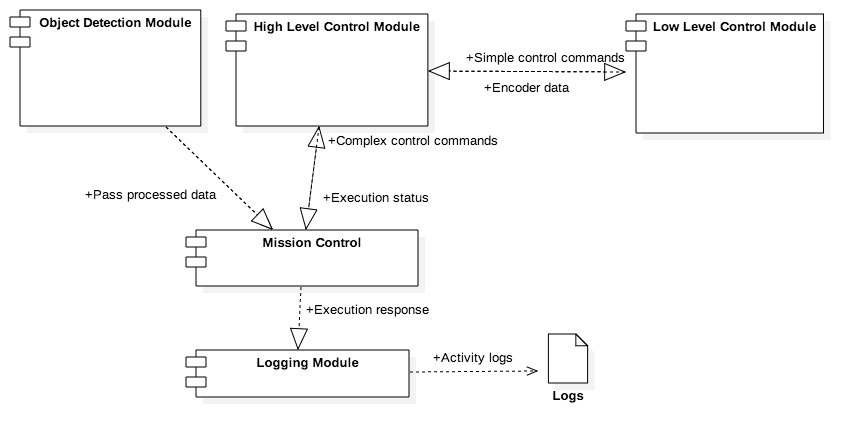
\includegraphics[scale=0.34]{assets/diagrams/ComponentDiagram.png}
%\caption{Shows how component are connected together.}
\end{figure}
\end{frame}

\begin{frame}
\frametitle{Class Diagram}
\end{frame}

%------------------------------------------------
\section{Algorithms}
%------------------------------------------------
\subsection{Transforms}
\begin{frame}
\frametitle{Hough Transform}
\begin{itemize}
\item Algorithm to detect imperfect instances of geometric shapes
\item Reduces the amount of data to be processes
\item Usage
\begin{itemize}
\item Detect outer walls and obstacles
\item Detect goal (Semi-Circle)
\end{itemize}
\item Idea (line detection case)
\begin{itemize}
\item Calculate the equation of the line through two consecutive points
\item Coefficients of the equation are added to a counter to record how many times the same equation is calculated
\item Coefficient calculated often equate to many points being roughly aligned	
\end{itemize}
\end{itemize}
\end{frame}

\begin{frame}
\frametitle{Hough Transform}
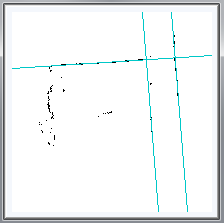
\includegraphics[scale=0.7]{assets/images/HoughTransform.png}
\end{frame}

\subsection{Bug Algorithms}
\begin{frame}
\frametitle{Bug algorithms}
\begin{itemize}
\item Knowledge of local environment and a global goal
\item Assumptions
\begin{itemize}
\item Known direction and distance to goal
\item Obstacle detection and encoder data
\item Finitely many obstacles in finite area
\end{itemize}
\item Idea
\begin{itemize}
\item Head towards goal
\item Follow obstacles until you can head towards goal again
\item Stop if there is no path to goal
\end{itemize}
\end{itemize}
\end{frame}

\begin{frame}
\frametitle{Bug Algorithms}
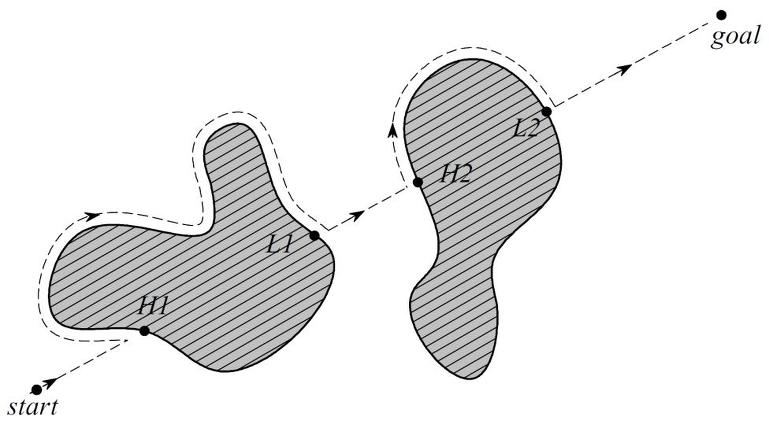
\includegraphics[scale=1]{assets/images/BugAlgorithms.jpg}
\end{frame}

\begin{frame}
\frametitle{(Modified) Bug algorithms}
\begin{itemize}
\item Missing assumptions
\begin{itemize}
\item Distance to goal is not known
\item Direction to goal might be imprecise(slippery surface, wrong encoder data)
\end{itemize}
\item Additional assumptions
\begin{itemize}
\item Environment has a rectangular shape
\end{itemize}
\item Greedy approach
\begin{itemize}
\item Head to the wall you are initially facing
\item Follow the walls until see the goal
\item Head to the goal
\end{itemize}
\end{itemize}
\end{frame}

\subsection{Filtering and Mapping}
\begin{frame}
\frametitle{Noise}
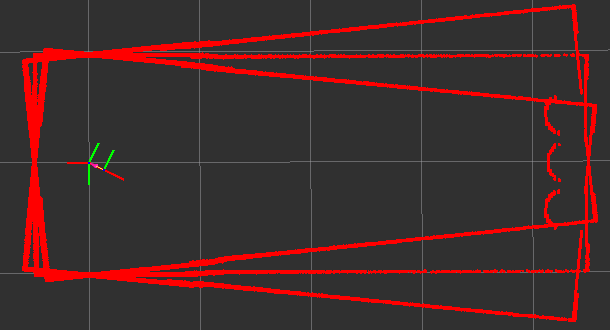
\includegraphics[scale=0.5]{assets/images/Noise.png}
\end{frame}

\begin{frame}
\frametitle{Kalman Filtering and Mapping}
\begin{itemize}
\item Kalman Filtering (Linear Quadratic Estimation)
\begin{itemize}
\item Input
\begin{itemize}
\item A series of measurements of a variable obtained over time
\item Observations contain statistical noise
\end{itemize}
\item Output
\begin{itemize}
\item Estimates of the values of the variable
\item These estimates tend to be more precise than one time measurements
\end{itemize}
\end{itemize}
\item Mapping
\begin{itemize}
\item Create a dynamic map of the surrounding environment
\item Use this map to reach the goal faster after the first iteration
\item Needs Kalman Filtering to get precise position of gaps, walls and goal
\end{itemize}
\end{itemize}



\end{frame}
%------------------------------------------------
\section{Design Patterns}
%------------------------------------------------
\subsection{Patterns in Use}
\begin{frame}
\frametitle{Singleton}
\end{frame}

\begin{frame}
\frametitle{Mediator}
\end{frame}
%------------------------------------------------
\section{Development Methodology}
%------------------------------------------------
\subsection{Workflow}
\begin{frame}
\frametitle{Stay Agile! Stay Alive!}
\begin{itemize}
\item Biweekly code sprints
\item Trello for task management and tracking backlog
\item Daily standups to keep track of progress and blockers
\item Weekly review and retrospective
\item Coordinated Pair programming sessions
\item End of sprint celebrations (Motivation!)
\end{itemize}
\end{frame}

\begin{frame}
\frametitle{Testing}
\begin{itemize}
\item Test Driven Development (TDD)
\begin{itemize}
\item Write tests before code
\item Helps clearly plan out program functionality
\item Reduces debug time drastically
\end{itemize}
\item Focused on four different domains:
\begin{itemize}
\item Unit Testing
\item Integration Testing 
\item System Testing
\item Stress Testing 
\end{itemize}
\end{itemize}
\end{frame}

\begin{frame}
\frametitle{Version Control}
\begin{itemize}
\item Git (using Github for remote)
\item Divide tasks into issues
\item Branching Model
\begin{itemize}
\item Each issue a separate branch on the remote
\item To be merged back in to the master after testing results
\end{itemize}
\end{itemize}
\end{frame}


%------------------------------------------------
\section{References}
%------------------------------------------------
\begin{frame}
\frametitle{References}
\footnotesize{
\begin{thebibliography}{99} % Beamer does not support BibTeX so references must be inserted manually as below
\bibitem[FRAVS, 2015]{p1} Andreea Ciuprina, Radu Homorozan, Jan Frederik Schaefer, Siddharth Shukla, Valentin Vasiliu (2015)
\newblock Social Network Clustering Project
\newblock \emph{Jacobs University Bremen}.

\bibitem[Tasgin, 2006]{p1} Mursel Tasgin and Haluk Bingol (2006)
\newblock Community Detection in Complex Networks using Genetic Algorithm
\newblock \emph{Department of Computer Engineering
Bogazici University, Istanbul, Turkey}.

\bibitem[Ochi, 2003]{p1} C. Rodrigo Dias and Luiz S. Ochi (2003)
\newblock Efficient Evolutionary Algorithms for the Clustering Problem in Directed Graphs
\newblock \emph{I.C. - Universidade Federal Fluminense}.


\bibitem[Neruda, 2013]{p1} Jan Kohout and Roman Neruda (2013)
\newblock Two-Phase Genetic Algorithm for Social Network Graphs Clustering
\newblock \emph{TG, Dept. of Computer Science and Engineering
Czech Technical University in Prague \& Institute of Computer Science
Academy of Sciences of the Czech Republic
Prague, The Czech Republic}.
\end{thebibliography}
}
\end{frame}

%----------------------------------------------------------------------------------------
\end{document} 
